%%
% Copyright (c) 2017 - 2021, Pascal Wagler;
% Copyright (c) 2014 - 2021, John MacFarlane
%
% All rights reserved.
%
% Redistribution and use in source and binary forms, with or without
% modification, are permitted provided that the following conditions
% are met:
%
% - Redistributions of source code must retain the above copyright
% notice, this list of conditions and the following disclaimer.
%
% - Redistributions in binary form must reproduce the above copyright
% notice, this list of conditions and the following disclaimer in the
% documentation and/or other materials provided with the distribution.
%
% - Neither the name of John MacFarlane nor the names of other
% contributors may be used to endorse or promote products derived
% from this software without specific prior written permission.
%
% THIS SOFTWARE IS PROVIDED BY THE COPYRIGHT HOLDERS AND CONTRIBUTORS
% "AS IS" AND ANY EXPRESS OR IMPLIED WARRANTIES, INCLUDING, BUT NOT
% LIMITED TO, THE IMPLIED WARRANTIES OF MERCHANTABILITY AND FITNESS
% FOR A PARTICULAR PURPOSE ARE DISCLAIMED. IN NO EVENT SHALL THE
% COPYRIGHT OWNER OR CONTRIBUTORS BE LIABLE FOR ANY DIRECT, INDIRECT,
% INCIDENTAL, SPECIAL, EXEMPLARY, OR CONSEQUENTIAL DAMAGES (INCLUDING,
% BUT NOT LIMITED TO, PROCUREMENT OF SUBSTITUTE GOODS OR SERVICES;
% LOSS OF USE, DATA, OR PROFITS; OR BUSINESS INTERRUPTION) HOWEVER
% CAUSED AND ON ANY THEORY OF LIABILITY, WHETHER IN CONTRACT, STRICT
% LIABILITY, OR TORT (INCLUDING NEGLIGENCE OR OTHERWISE) ARISING IN
% ANY WAY OUT OF THE USE OF THIS SOFTWARE, EVEN IF ADVISED OF THE
% POSSIBILITY OF SUCH DAMAGE.
%%

%%
% This is the Eisvogel pandoc LaTeX template.
%
% For usage information and examples visit the official GitHub page:
% https://github.com/Wandmalfarbe/pandoc-latex-template
%%

% Options for packages loaded elsewhere
\PassOptionsToPackage{unicode}{hyperref}
\PassOptionsToPackage{hyphens}{url}
\PassOptionsToPackage{dvipsnames,svgnames*,x11names*,table}{xcolor}
%
\documentclass[
  english,
  paper=a4,
  ,captions=tableheading
]{scrartcl}
\usepackage{amsmath,amssymb}
\usepackage{lmodern}
\usepackage{setspace}
\setstretch{1.2}
\usepackage{ifxetex,ifluatex}
\ifnum 0\ifxetex 1\fi\ifluatex 1\fi=0 % if pdftex
  \usepackage[T1]{fontenc}
  \usepackage[utf8]{inputenc}
  \usepackage{textcomp} % provide euro and other symbols
\else % if luatex or xetex
  \usepackage{unicode-math}
  \defaultfontfeatures{Scale=MatchLowercase}
  \defaultfontfeatures[\rmfamily]{Ligatures=TeX,Scale=1}
\fi
% Use upquote if available, for straight quotes in verbatim environments
\IfFileExists{upquote.sty}{\usepackage{upquote}}{}
\IfFileExists{microtype.sty}{% use microtype if available
  \usepackage[]{microtype}
  \UseMicrotypeSet[protrusion]{basicmath} % disable protrusion for tt fonts
}{}
\makeatletter
\@ifundefined{KOMAClassName}{% if non-KOMA class
  \IfFileExists{parskip.sty}{%
    \usepackage{parskip}
  }{% else
    \setlength{\parindent}{0pt}
    \setlength{\parskip}{6pt plus 2pt minus 1pt}}
}{% if KOMA class
  \KOMAoptions{parskip=half}}
\makeatother
\usepackage{xcolor}
\definecolor{default-linkcolor}{HTML}{A50000}
\definecolor{default-filecolor}{HTML}{A50000}
\definecolor{default-citecolor}{HTML}{4077C0}
\definecolor{default-urlcolor}{HTML}{4077C0}
\IfFileExists{xurl.sty}{\usepackage{xurl}}{} % add URL line breaks if available
\IfFileExists{bookmark.sty}{\usepackage{bookmark}}{\usepackage{hyperref}}
\hypersetup{
  pdftitle={Example PDF},
  pdfauthor={Author},
  pdflang={en},
  pdfsubject={Markdown},
  pdfkeywords={Markdown, Example},
  hidelinks,
  breaklinks=true,
  pdfcreator={LaTeX via pandoc with the Eisvogel template}}
\urlstyle{same} % disable monospaced font for URLs
\usepackage[margin=2.5cm,includehead=true,includefoot=true,centering,]{geometry}
\usepackage{listings}
\newcommand{\passthrough}[1]{#1}
\lstset{defaultdialect=[5.3]Lua}
\lstset{defaultdialect=[x86masm]Assembler}
\usepackage{longtable,booktabs,array}
\usepackage{calc} % for calculating minipage widths
% Correct order of tables after \paragraph or \subparagraph
\usepackage{etoolbox}
\makeatletter
\patchcmd\longtable{\par}{\if@noskipsec\mbox{}\fi\par}{}{}
\makeatother
% Allow footnotes in longtable head/foot
\IfFileExists{footnotehyper.sty}{\usepackage{footnotehyper}}{\usepackage{footnote}}
\makesavenoteenv{longtable}
% add backlinks to footnote references, cf. https://tex.stackexchange.com/questions/302266/make-footnote-clickable-both-ways
\usepackage{footnotebackref}
\usepackage{graphicx}
\makeatletter
\def\maxwidth{\ifdim\Gin@nat@width>\linewidth\linewidth\else\Gin@nat@width\fi}
\def\maxheight{\ifdim\Gin@nat@height>\textheight\textheight\else\Gin@nat@height\fi}
\makeatother
% Scale images if necessary, so that they will not overflow the page
% margins by default, and it is still possible to overwrite the defaults
% using explicit options in \includegraphics[width, height, ...]{}
\setkeys{Gin}{width=\maxwidth,height=\maxheight,keepaspectratio}
% Set default figure placement to htbp
\makeatletter
\def\fps@figure{htbp}
\makeatother
\setlength{\emergencystretch}{3em} % prevent overfull lines
\providecommand{\tightlist}{%
  \setlength{\itemsep}{0pt}\setlength{\parskip}{0pt}}
\setcounter{secnumdepth}{-\maxdimen} % remove section numbering

% Make use of float-package and set default placement for figures to H.
% The option H means 'PUT IT HERE' (as  opposed to the standard h option which means 'You may put it here if you like').
\usepackage{float}
\floatplacement{figure}{H}

\ifxetex
    % See issue https://github.com/reutenauer/polyglossia/issues/127
  \renewcommand*\familydefault{\sfdefault}
    % Load polyglossia as late as possible: uses bidi with RTL langages (e.g. Hebrew, Arabic)
  \usepackage{polyglossia}
  \setmainlanguage[]{english}
\else
  \usepackage[main=english]{babel}
% get rid of language-specific shorthands (see #6817):
\let\LanguageShortHands\languageshorthands
\def\languageshorthands#1{}
\fi
\ifluatex
  \usepackage{selnolig}  % disable illegal ligatures
\fi

\title{Example PDF}
\author{Author}
\date{2017-02-20}



%%
%% added
%%

%
% language specification
%
% If no language is specified, use English as the default main document language.
%



%
% for the background color of the title page
%

%
% break urls
%
\PassOptionsToPackage{hyphens}{url}

%
% When using babel or polyglossia with biblatex, loading csquotes is recommended
% to ensure that quoted texts are typeset according to the rules of your main language.
%
\usepackage{csquotes}

%
% captions
%
\definecolor{caption-color}{HTML}{777777}
\usepackage[font={stretch=1.2}, textfont={color=caption-color}, position=top, skip=4mm, labelfont=bf, singlelinecheck=false, justification=raggedright]{caption}
\setcapindent{0em}

%
% blockquote
%
\definecolor{blockquote-border}{RGB}{221,221,221}
\definecolor{blockquote-text}{RGB}{119,119,119}
\usepackage{mdframed}
\newmdenv[rightline=false,bottomline=false,topline=false,linewidth=3pt,linecolor=blockquote-border,skipabove=\parskip]{customblockquote}
\renewenvironment{quote}{\begin{customblockquote}\list{}{\rightmargin=0em\leftmargin=0em}%
\item\relax\color{blockquote-text}\ignorespaces}{\unskip\unskip\endlist\end{customblockquote}}

%
% Source Sans Pro as the de­fault font fam­ily
% Source Code Pro for monospace text
%
% 'default' option sets the default
% font family to Source Sans Pro, not \sfdefault.
%
\ifnum 0\ifxetex 1\fi\ifluatex 1\fi=0 % if pdftex
    \usepackage[default]{sourcesanspro}
  \usepackage{sourcecodepro}
  \else % if not pdftex
    \usepackage[default]{sourcesanspro}
  \usepackage{sourcecodepro}

  % XeLaTeX specific adjustments for straight quotes: https://tex.stackexchange.com/a/354887
  % This issue is already fixed (see https://github.com/silkeh/latex-sourcecodepro/pull/5) but the
  % fix is still unreleased.
  % TODO: Remove this workaround when the new version of sourcecodepro is released on CTAN.
  \ifxetex
    \makeatletter
    \defaultfontfeatures[\ttfamily]
      { Numbers   = \sourcecodepro@figurestyle,
        Scale     = \SourceCodePro@scale,
        Extension = .otf }
    \setmonofont
      [ UprightFont    = *-\sourcecodepro@regstyle,
        ItalicFont     = *-\sourcecodepro@regstyle It,
        BoldFont       = *-\sourcecodepro@boldstyle,
        BoldItalicFont = *-\sourcecodepro@boldstyle It ]
      {SourceCodePro}
    \makeatother
  \fi
  \fi

%
% heading color
%
\definecolor{heading-color}{RGB}{40,40,40}
\addtokomafont{section}{\color{heading-color}}
% When using the classes report, scrreprt, book,
% scrbook or memoir, uncomment the following line.
%\addtokomafont{chapter}{\color{heading-color}}

%
% variables for title, author and date
%
\usepackage{titling}
\title{Example PDF}
\author{Author}
\date{2017-02-20}

%
% tables
%

\definecolor{table-row-color}{HTML}{F5F5F5}
\definecolor{table-rule-color}{HTML}{999999}

%\arrayrulecolor{black!40}
\arrayrulecolor{table-rule-color}     % color of \toprule, \midrule, \bottomrule
\setlength\heavyrulewidth{0.3ex}      % thickness of \toprule, \bottomrule
\renewcommand{\arraystretch}{1.3}     % spacing (padding)


%
% remove paragraph indention
%
\setlength{\parindent}{0pt}
\setlength{\parskip}{6pt plus 2pt minus 1pt}
\setlength{\emergencystretch}{3em}  % prevent overfull lines

%
%
% Listings
%
%


%
% general listing colors
%
\definecolor{listing-background}{HTML}{F7F7F7}
\definecolor{listing-rule}{HTML}{B3B2B3}
\definecolor{listing-numbers}{HTML}{B3B2B3}
\definecolor{listing-text-color}{HTML}{000000}
\definecolor{listing-keyword}{HTML}{435489}
\definecolor{listing-keyword-2}{HTML}{1284CA} % additional keywords
\definecolor{listing-keyword-3}{HTML}{9137CB} % additional keywords
\definecolor{listing-identifier}{HTML}{435489}
\definecolor{listing-string}{HTML}{00999A}
\definecolor{listing-comment}{HTML}{8E8E8E}

\lstdefinestyle{eisvogel_listing_style}{
  language         = java,
  numbers          = left,
  xleftmargin      = 2.7em,
  framexleftmargin = 2.5em,
  backgroundcolor  = \color{listing-background},
  basicstyle       = \color{listing-text-color}\linespread{1.0}\small\ttfamily{},
  breaklines       = true,
  frame            = single,
  framesep         = 0.19em,
  rulecolor        = \color{listing-rule},
  frameround       = ffff,
  tabsize          = 4,
  numberstyle      = \color{listing-numbers},
  aboveskip        = 1.0em,
  belowskip        = 0.1em,
  abovecaptionskip = 0em,
  belowcaptionskip = 1.0em,
  keywordstyle     = {\color{listing-keyword}\bfseries},
  keywordstyle     = {[2]\color{listing-keyword-2}\bfseries},
  keywordstyle     = {[3]\color{listing-keyword-3}\bfseries\itshape},
  sensitive        = true,
  identifierstyle  = \color{listing-identifier},
  commentstyle     = \color{listing-comment},
  stringstyle      = \color{listing-string},
  showstringspaces = false,
  escapeinside     = {/*@}{@*/}, % Allow LaTeX inside these special comments
  literate         =
  {á}{{\'a}}1 {é}{{\'e}}1 {í}{{\'i}}1 {ó}{{\'o}}1 {ú}{{\'u}}1
  {Á}{{\'A}}1 {É}{{\'E}}1 {Í}{{\'I}}1 {Ó}{{\'O}}1 {Ú}{{\'U}}1
  {à}{{\`a}}1 {è}{{\'e}}1 {ì}{{\`i}}1 {ò}{{\`o}}1 {ù}{{\`u}}1
  {À}{{\`A}}1 {È}{{\'E}}1 {Ì}{{\`I}}1 {Ò}{{\`O}}1 {Ù}{{\`U}}1
  {ä}{{\"a}}1 {ë}{{\"e}}1 {ï}{{\"i}}1 {ö}{{\"o}}1 {ü}{{\"u}}1
  {Ä}{{\"A}}1 {Ë}{{\"E}}1 {Ï}{{\"I}}1 {Ö}{{\"O}}1 {Ü}{{\"U}}1
  {â}{{\^a}}1 {ê}{{\^e}}1 {î}{{\^i}}1 {ô}{{\^o}}1 {û}{{\^u}}1
  {Â}{{\^A}}1 {Ê}{{\^E}}1 {Î}{{\^I}}1 {Ô}{{\^O}}1 {Û}{{\^U}}1
  {œ}{{\oe}}1 {Œ}{{\OE}}1 {æ}{{\ae}}1 {Æ}{{\AE}}1 {ß}{{\ss}}1
  {ç}{{\c c}}1 {Ç}{{\c C}}1 {ø}{{\o}}1 {å}{{\r a}}1 {Å}{{\r A}}1
  {€}{{\EUR}}1 {£}{{\pounds}}1 {«}{{\guillemotleft}}1
  {»}{{\guillemotright}}1 {ñ}{{\~n}}1 {Ñ}{{\~N}}1 {¿}{{?`}}1
  {…}{{\ldots}}1 {≥}{{>=}}1 {≤}{{<=}}1 {„}{{\glqq}}1 {“}{{\grqq}}1
  {”}{{''}}1
}
\lstset{style=eisvogel_listing_style}

%
% Java (Java SE 12, 2019-06-22)
%
\lstdefinelanguage{Java}{
  morekeywords={
    % normal keywords (without data types)
    abstract,assert,break,case,catch,class,continue,default,
    do,else,enum,exports,extends,final,finally,for,if,implements,
    import,instanceof,interface,module,native,new,package,private,
    protected,public,requires,return,static,strictfp,super,switch,
    synchronized,this,throw,throws,transient,try,volatile,while,
    % var is an identifier
    var
  },
  morekeywords={[2] % data types
    % primitive data types
    boolean,byte,char,double,float,int,long,short,
    % String
    String,
    % primitive wrapper types
    Boolean,Byte,Character,Double,Float,Integer,Long,Short
    % number types
    Number,AtomicInteger,AtomicLong,BigDecimal,BigInteger,DoubleAccumulator,DoubleAdder,LongAccumulator,LongAdder,Short,
    % other
    Object,Void,void
  },
  morekeywords={[3] % literals
    % reserved words for literal values
    null,true,false,
  },
  sensitive,
  morecomment  = [l]//,
  morecomment  = [s]{/*}{*/},
  morecomment  = [s]{/**}{*/},
  morestring   = [b]",
  morestring   = [b]',
}

\lstdefinelanguage{XML}{
  morestring      = [b]",
  moredelim       = [s][\bfseries\color{listing-keyword}]{<}{\ },
  moredelim       = [s][\bfseries\color{listing-keyword}]{</}{>},
  moredelim       = [l][\bfseries\color{listing-keyword}]{/>},
  moredelim       = [l][\bfseries\color{listing-keyword}]{>},
  morecomment     = [s]{<?}{?>},
  morecomment     = [s]{<!--}{-->},
  commentstyle    = \color{listing-comment},
  stringstyle     = \color{listing-string},
  identifierstyle = \color{listing-identifier}
}

%
% header and footer
%
\usepackage[headsepline,footsepline]{scrlayer-scrpage}

\newpairofpagestyles{eisvogel-header-footer}{
  \clearpairofpagestyles
  \ihead[2017-02-20]{Example PDF}
  \chead[]{}
  \ohead[Example PDF]{2017-02-20}
  \ifoot[\thepage]{Author}
  \cfoot[]{}
  \ofoot[Author]{\thepage}
  \addtokomafont{pageheadfoot}{\upshape}
}
\pagestyle{eisvogel-header-footer}

%%
%% end added
%%

\begin{document}

%%
%% begin titlepage
%%

%%
%% end titlepage
%%



\hypertarget{atomicchessos}{%
\section{AtomicChessOS}\label{atomicchessos}}

\hypertarget{atc-controller}{%
\section{ATC CONTROLLER}\label{atc-controller}}

The controller is the main system on the embedded device that controls
the hardware of a ATC Table

\begin{itemize}
\tightlist
\item
  Motor Control
\item
  Communcication with the Server
\item
  Communication with the UI running on the device
\item
  Chess Figure Movement Algorithm
\end{itemize}

For this software component, we are using a Windows and Visual Studi
environment for developing the software. Our embedded system is a linux
device, so we have to build the application for the linux environment
running on the emmbedded device. For this task, the prevously build
buildroot toolchain is used. A software plugin called VisualGDB for
Visual Studio, enable Visual Studio to use the linux toolchain over a
remote linux system, in order to build and deploy the application.

\hypertarget{requirements}{%
\subsection{REQUIREMENTS}\label{requirements}}

\begin{itemize}
\tightlist
\item
  windows pc for development
\item
  linux pc with buildroot toolchain
\item
  embedded system for deployment
\end{itemize}

\hypertarget{setup-a-project-using-visual-studio-and-visualgdb}{%
\subsection{SETUP A PROJECT USING VISUAL STUDIO AND
VisualGDB}\label{setup-a-project-using-visual-studio-and-visualgdb}}

\hypertarget{requirements-1}{%
\subsubsection{REQUIREMENTS}\label{requirements-1}}

On the development windows pc is the following software installed: *
Windows 10 Pro x64 * Visual Studio 2019 (Community or Enterprise) *
VisualGDB Plugin (Version 5.5, Linux Edition) * A SSH Client (MobaXterm
Personal Edition) * git (Gitkraken)

\hypertarget{linux-build-system}{%
\subsubsection{LINUX BUILD SYSTEM}\label{linux-build-system}}

On the linux build system, the VisualGSB plugin builds the project. The
system is a \passthrough{\lstinline!Intel Nuc 10!}, mini pc, with a
stock \passthrough{\lstinline!Ubuntu 20.04!} installed. One the machine
are all package requirements for building the buildroot toolchain
installed (see buildroot chapter).

After cloning the repository
\passthrough{\lstinline!$ git clone -b buildroot git@github.com:RBEGamer/AtomicChessOS.git ./atc\_buildroot!}
and switched to the \passthrough{\lstinline!buildroot!} branch, the
build process of the toolchain was invoked using the build script
\passthrough{\lstinline!$ ./atc\_buildroot/src/src\_buildroot/buildroot/build.sh!}.

After building the toolchain is completed, the further configuration
work can be done on the windows development pc. Its nessessary for the
linux build system to allow SSH connections. Its may required to install
the OpenSSHServer uisng
\passthrough{\lstinline!$ sudo apt install openssh-server!}.

The VisualGDB plugin requires some extra packages on the build pc:

\begin{itemize}
\tightlist
\item
  \passthrough{\lstinline!$ sudo apt-get install socat!}
\end{itemize}

Now the configuration of the linux build pc for the VisualGDB plugin is
complete. The next step, is the setup of the embedded system for
deployment.

\hypertarget{embedded-system-deployment}{%
\subsubsection{EMBEDDED SYSTEM
DEPLOYMENT}\label{embedded-system-deployment}}

Afer building the sources into an executable, the final binaries will be
copied to the embedded system. The embedded system is flashed with tha
latest image build by buildroot.

In order to setup the VisualGDB Project, its nessessary that the
embedded device can be accessed over SSH.

\hypertarget{makefile-modifications}{%
\paragraph{MAKEFILE MODIFICATIONS}\label{makefile-modifications}}

\begin{itemize}
\tightlist
\item
  buildroot build oveerrides TARGETNAME AND CONFIG to load a different
  makefile config in order to use the toolchain generated by buildroot
  The different configurationa are stored in different .mk files that
  will be includes by the Makefile. THe
  \passthrough{\lstinline!debug.mk!} configuration contains theVisualGDB
  Configuration that allows the Visual Studio Plugin to use the remote
  toolchain on the linux server and can only build by over the visual
  gdb plugin. The \passthrough{\lstinline!release.mk!} configuration is
  used to build the controller apllication with the buildroot framework.
  It used the compiler executable paths defines by \$CC. \$LD enviroment
  variables and build the program with release flags and without any
  debug symbols. All used libraries are linked staticly.
\end{itemize}

\hypertarget{third-party-libraries}{%
\subsection{THIRD PARTY LIBRARIES}\label{third-party-libraries}}

The ATC\_Controller software uses serveral different third party
libraries, escacially for http requests and json parsing. *
\passthrough{\lstinline!https://github.com/nlohmann/json#serialization--deserialization!},
json parsing. *
\passthrough{\lstinline!https://github.com/yhirose/cpp-httplib!},
http/https requests. *
\passthrough{\lstinline!https://github.com/Neargye/magic\_enum!}, enum
handling. * \passthrough{\lstinline!https://github.com/emilk/loguru!} A
copy of the used versions, are located in the controller software
directory.

\hypertarget{controller-overview}{%
\section{CONTROLLER OVERVIEW}\label{controller-overview}}

\hypertarget{motor-driver}{%
\subsection{MOTOR DRIVER}\label{motor-driver}}

\hypertarget{board-class}{%
\subsection{BOARD CLASS}\label{board-class}}

\hypertarget{chess-piece}{%
\subsection{CHESS PIECE}\label{chess-piece}}

\hypertarget{nfc-tag-content-generator}{%
\subsubsection{NFC TAG CONTENT
GENERATOR}\label{nfc-tag-content-generator}}

Each figures NFC tag is ued to identify the figure. For easy usage of
the NFC tag, it is formatted into the NDEF format, so its simply
possible to program the NFC tags with an mobile phone. The tag contains
a ndef \passthrough{\lstinline!text record!} with a string to identifiy
the type of figure (three bits), color (one bit) and a counting number
(four bits). A combination of all three attributes make the figures id
unique to the system. For the automatic unique ID generation, a html
page \passthrough{\lstinline!ChessFigureIDGenerator.html!} was created
to automaticliy generate all ID for a complete chess board. Only one
byte is stored in the record of the text record and so only 10bytes are
used on the NFC tag.

\begin{itemize}
\tightlist
\item
  MSB {[}7,6,5,4,3,2,1,0{]} LSB
\item
  MSB {[}TYPE,TYPE,TYPE,COLOR,ID,ID,ID,ID{]} LSB
\end{itemize}

For reading the NFC tag with the PN532, the program only reads the first
NDEF record and parses the text record data to get the figure type. With
this system it is possible to expand the system further and store more
data on the NFC tag, by adding more NDEF records.

On the controller side two functions were created to generate the unique
ids and read them back.

\begin{lstlisting}[language={C++}]
  ChessPiece::FIGURE fig;
    fig.figure_number = 1;
    fig.color = ChessPiece::COLOR_BLACK;
    fig.type = ChessPiece::TYPE_KNIGHT;
  
  //GENERATE ID FROM STRUCT
  uint8_t UNIQUE_ID = ChessPiece::figure2NDEF(fig);
  
  //PARSE UNIQUE_ID BACK TO A STRUCT
  ChessPiece::FIGURE back = ChessPiece::NDEF2Figure(UNIQUE_ID);
  
\end{lstlisting}

\begin{itemize}
\tightlist
\item
  IMAGE
\end{itemize}

\hypertarget{config-and-calibration}{%
\subsection{CONFIG AND CALIBRATION}\label{config-and-calibration}}

The system uses a config file located in the filesystem
\passthrough{\lstinline!/usr/ATC/atccontroller.ini!}.

\hypertarget{calibration}{%
\subsubsection{CALIBRATION}\label{calibration}}

In order to calibrate the mechanic, several entries in the config file
has to be changed.

\begin{figure}
\centering
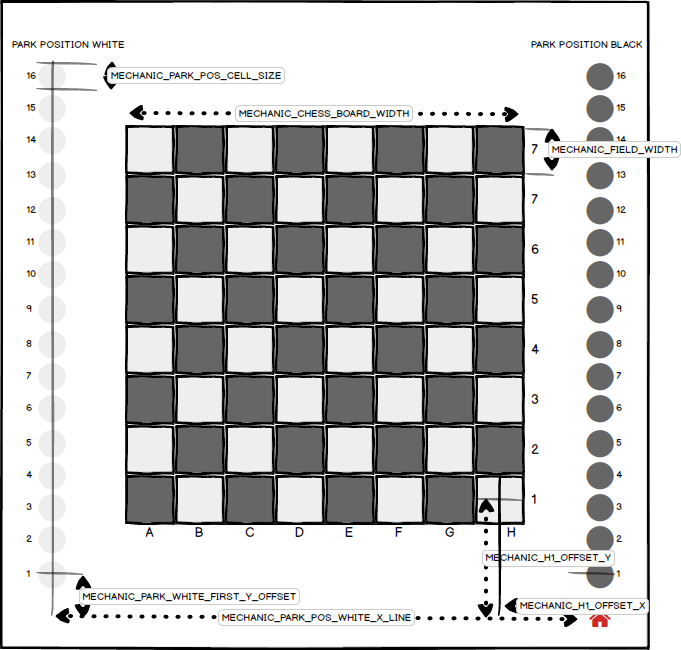
\includegraphics{./images/ATC_Calibration_Guide.png}
\caption{MOCKUP\_MAIN\_MENU}
\end{figure}

\hypertarget{chess-piece-movement-algorithm}{%
\subsubsection{Chess Piece Movement
Algorithm}\label{chess-piece-movement-algorithm}}

\begin{figure}
\centering
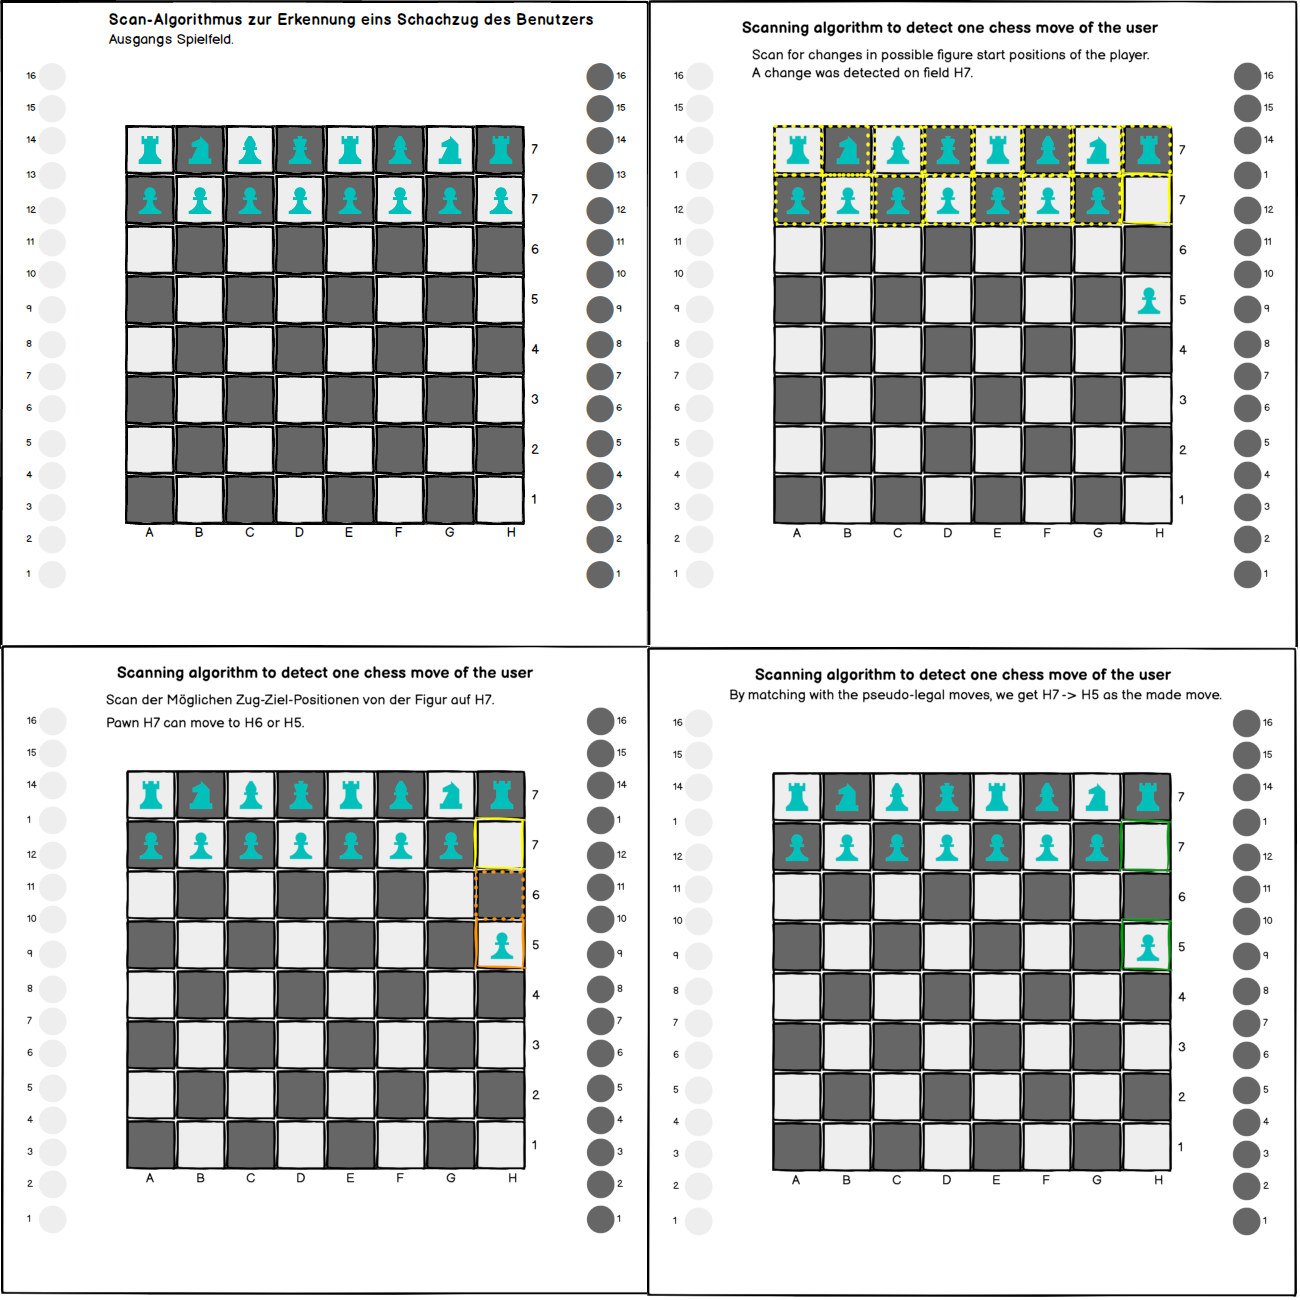
\includegraphics{./images/ATC_ChessMoveAlgorithm.png}
\caption{MOCKUP\_MAIN\_MENU}
\end{figure}

\hypertarget{basic-movement-procedure}{%
\paragraph{BASIC MOVEMENT PROCEDURE}\label{basic-movement-procedure}}

*move \#\#\#\#\# BOARD \textless{}-\textgreater{} BOARD

\hypertarget{park_position---board-board---park_positon}{%
\subparagraph{PARK\_POSITION \textless{}-\textgreater{} BOARD
\textbar{}\textbar{} BOARD \textless{}-\textgreater{}
PARK\_POSITON}\label{park_position---board-board---park_positon}}

\hypertarget{algorithm-improvements}{%
\subparagraph{ALGORITHM IMPROVEMENTS}\label{algorithm-improvements}}

\begin{itemize}
\item
  queue movement all movementinstructions needed for a move, send them
  combinded to the motor driver
\item
  send coil change event only if changed, SPI Implementation needs time
  (about 0.5 Secs with the wait ACK)
\item
\end{itemize}

\hypertarget{piece-move-time}{%
\paragraph{PIECE MOVE TIME}\label{piece-move-time}}

\begin{longtable}[]{@{}lll@{}}
\toprule
\begin{minipage}[b]{0.29\columnwidth}\raggedright
ALGORITHM\_V1\_TRAVEL\_TIME {[}s{]}\strut
\end{minipage} & \begin{minipage}[b]{0.29\columnwidth}\raggedright
ALGORITHM\_V2\_TRAVEL\_TIME {[}s{]}\strut
\end{minipage} & \begin{minipage}[b]{0.34\columnwidth}\raggedright
TRAVEL\_DISTANCE {[}FIELDS\_DIAGONAL{]}\strut
\end{minipage}\tabularnewline
\midrule
\endhead
\begin{minipage}[t]{0.29\columnwidth}\raggedright
7.20\strut
\end{minipage} & \begin{minipage}[t]{0.29\columnwidth}\raggedright
2.56\strut
\end{minipage} & \begin{minipage}[t]{0.34\columnwidth}\raggedright
1\strut
\end{minipage}\tabularnewline
\begin{minipage}[t]{0.29\columnwidth}\raggedright
11.56\strut
\end{minipage} & \begin{minipage}[t]{0.29\columnwidth}\raggedright
6,20\strut
\end{minipage} & \begin{minipage}[t]{0.34\columnwidth}\raggedright
3\strut
\end{minipage}\tabularnewline
\begin{minipage}[t]{0.29\columnwidth}\raggedright
12,27\strut
\end{minipage} & \begin{minipage}[t]{0.29\columnwidth}\raggedright
7,06\strut
\end{minipage} & \begin{minipage}[t]{0.34\columnwidth}\raggedright
5\strut
\end{minipage}\tabularnewline
\begin{minipage}[t]{0.29\columnwidth}\raggedright
14,39\strut
\end{minipage} & \begin{minipage}[t]{0.29\columnwidth}\raggedright
6,56\strut
\end{minipage} & \begin{minipage}[t]{0.34\columnwidth}\raggedright
8\strut
\end{minipage}\tabularnewline
\bottomrule
\end{longtable}

\begin{figure}
\centering
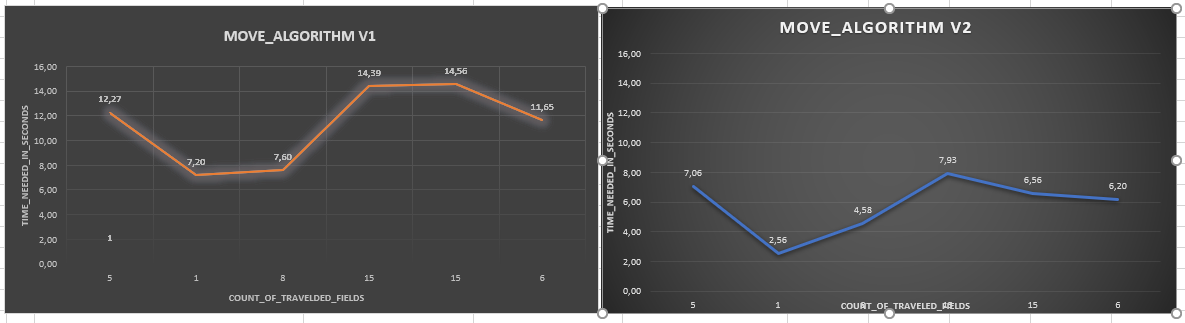
\includegraphics{./images/FigureMovementTims_GRAPH_COMP.PNG}
\caption{MOCKUP\_MAIN\_MENU}
\end{figure}

\hypertarget{movement-speed-comarpision-hardware-v1-v2}{%
\subsubsection{MOVEMENT SPEED COMARPISION HARDWARE V1 /
V2}\label{movement-speed-comarpision-hardware-v1-v2}}

\begin{itemize}
\tightlist
\item
  gocde slower nicht
\end{itemize}

\hypertarget{linux-handling-different}{%
\paragraph{{[}LINUX{]} HANDLING
DIFFERENT}\label{linux-handling-different}}

The simplified hardware design of the projects uses two USB2Serial
adapters to connect the SKR1.3 Stepper Driver Board and the User-Move
Dector with the Embedded System. All serial deives will be mount under
the \passthrough{\lstinline!/dev/ttyXXX!} path and the the squence can
be differ after each reboot. In order to prevent this, it is possible to
mount a usb device with a Vendor and Product-ID to a specified path
using a custom udev roule. For each rule, the Vendor and Product-ID is
needed, for this commands like \passthrough{\lstinline!lsub!} or
\passthrough{\lstinline!usb-devices!} and output the relevant
information for each usb device attached.

\begin{lstlisting}
$ usb-devices

T:  Bus=03 Lev=02 Prnt=02 Port=02 Cnt=03 Dev#= 11 Spd=12  MxCh= 0
D:  Ver= 2.00 Cls=ef(misc ) Sub=02 Prot=01 MxPS=64 #Cfgs=  1
P:  Vendor=1d50 ProdID=6029 Rev=01.00
S:  Manufacturer=marlinfw.org 
S:  Product=Marlin USB Device
S:  SerialNumber=06FF800AAF3D08075C664F58F50020C3
C:  #Ifs= 3 Cfg#= 1 Atr=80 MxPwr=500mA
I:  If#=0x0 Alt= 0 #EPs= 1 Cls=02(commc) Sub=02 Prot=00 Driver=cdc_acm
I:  If#=0x1 Alt= 0 #EPs= 2 Cls=0a(data ) Sub=00 Prot=00 Driver=cdc_acm
I:  If#=0x2 Alt= 0 #EPs= 2 Cls=08(stor.) Sub=06 Prot=50 Driver=usb-storage
\end{lstlisting}

During development, several different board are used to control the
different hardware sections. These can be divided into two main groups :

\begin{itemize}
\tightlist
\item
  \passthrough{\lstinline!Stepper-Controller!} - For controlling the
  Stpper-Drivers, Endstop, Coils/Servo
\item
  \passthrough{\lstinline!User-Move-Detector!} - To interface the
  hall-sensor array, to detect a manual move of the figures.
\end{itemize}

In the following table, the Vendor/Product-IDs from some tested boards
are listed below:

\begin{longtable}[]{@{}llllll@{}}
\toprule
Product & SUBSYSTEM & Vendor-ID & Product-ID & SYMLINK &
Board-Type\tabularnewline
\midrule
\endhead
Bigtreetech SKR 1.4 Turbo & tty & 1d50 & 6029 & ttySKR &
Stepper-Controller\tabularnewline
Bigtreetech SKR 1.3 & tty & 1d50 & 6029 & ttySKR &
Stepper-Controller\tabularnewline
Arduino Due {[}Programming Port{]} & tty & 2341 & 003d & ttyUBC &
User-Move-Detector\tabularnewline
Arduino Due {[}Native SAMX3 Port{]} & tty & 2341 & 003e & ttyUBC &
User-Move-Detector\tabularnewline
CH340 & tty & 1a86 & 7523 & ttyUBC & User-Move-Detector\tabularnewline
HL-340 & tty & 1a86 & 7523 & ttyUBC & User-Move-Detector\tabularnewline
STM32F411 & tty & 0483 & 5740 & ttyUBC &
User-Move-Detector\tabularnewline
\bottomrule
\end{longtable}

With these information, is is possible to generate the needed udev
rules.

\begin{lstlisting}
$ cat /etc/udev/rules.d/50-usb.rules

...
SUBSYSTEM=="tty", ATTRS{idVendor}=="1d50", ATTRS{idProduct}=="6029", SYMLINK+="ttySKR"
...
SUBSYSTEM=="tty", ATTRS{idVendor}=="0483", ATTRS{idProduct}=="5740", SYMLINK+="ttyUBC"
...
\end{lstlisting}

This configuration archieves, that any type (of supported)
Stepper-Controller-Boards are accessable over the
\passthrough{\lstinline!/dev/ttySKR!} symblink.

After the installation of the rules and connection of a SKR1.3 and a
STM32F411 (known as STM32-BlackPill), the device directory contains the
following entires:

\begin{lstlisting}
ls /dev/tty*

/dev/ttyS27  /dev/ttyS6
/dev/ttyUSB0  /dev/ttyACMA0  /dev/tty25  /dev/tty32  /dev/tty4  /dev/ttyprintk  /dev/ttySKR  /dev/ttyUBC
\end{lstlisting}

The in the configutation file of the controller file, these tty paths
are set and no reconfiguration for different hardware configuration is
needed.

\end{document}
